% ======================================================================
\documentclass[12pt,twoside,letterpaper]{article}

%%%%%%%%%%%%%%%%%%%%%%%%%%%%%%%%%%%%%%%
% Jianrong Deng @ 20171211 
% This is an analysis note on high energy cosmic rays selection on CCD
% images of LAMOST. 
%%%%%%%%%%%%%%%%%%%%%%%%%%%%%%%%%%%%%%%


\usepackage{epsfig}

% ======================================================================
\begin{document}


% ======================================================================
% Title and author
\begin{center}
  \begin{Large}
  {\bf High Energy Cosmic Rays Found on the LAMOST CCDs}
  \end{Large}
\end{center}

\begin{center}
\small{Jianjun Chen, Jianrong Deng}\vspace{1.0ex} \\
\emph{NAOC, CAS}
\end{center}
% ======================================================================


% ======================================================================
\begin{abstract}

\end{abstract}
% ======================================================================

% ======================================================================
\section{Motivation} 
% ======================================================================

% ======================================================================
\subsection{Ultra High Energy Cosmic Rays} 
% ======================================================================

% ======================================================================
\section{Introduction} 
% ======================================================================

% ======================================================================
\subsection{Current Status} 
% ======================================================================


% ======================================================================
\section{Detector} 
% ======================================================================

% ======================================================================
\subsection{The LAMOST Telescope} 
% ======================================================================

% ======================================================================
%\subsection{The CCD Cameras of the LAMOST Telescope\cite{}UCAM-CCD} 
\subsection{The CCD Cameras of the LAMOST Telescope} 
% ======================================================================

The LAMOST Charge-Coupled Device (CCD):
 %"back illuminated CCD with 4K by 4K pixels and 12 x 12 um pixel size, supporting for four output readout mode. LAMOST UCAM controller uses two of the four output amplifiers for output images. By liquid nitrogen cooling, the working temperature of the e2v CCD reached -130C. "
       \begin{itemize}
           \item 32 CCDs
	   \item 16 for Blue band 
	   \item 16 for Red  band
	   \item Cooling:
	   \begin{itemize}
	       \item Liquid Nitrogen cooling
	       \item at ${-130^{0}}$ Celsius
	   \end{itemize}
	   \item e2v 203-82 
	   \begin{itemize}
	       \item back illuminated CCD
	       \item 4K by 4K pixels
	       \item 12 x 12 micron pixel size
	       \item flatness better than 15 micron with 100\% active area 
	       \item support 4 output readout modes?
	       \item LAMOST uses two  of the four amplifiers to generate output images
	   \end{itemize}
       \end{itemize}



% ======================================================================
\section{Online Data Taking / Observation} 
% ======================================================================

% ======================================================================
\section{Offline Data Analysis -- Bias Data} 
% ======================================================================

The analysis package is developed using Python language. 

% ======================================================================
\subsection{Raw Data Format} 
% ======================================================================

The raw data is available in Fits format, which can be read out using
the astropy.io module with a couple simple lines, such as

def read\_fits (filename): \\
   \hspace{0.5cm}from astropy.io import fits \\
   \hspace{0.5cm}return fits.getdata(filename, ext=0) \\

Where:

       \begin{itemize}
           \item filename: input data
           \item output data: raw data matrix
       \end{itemize}
Note: the "ext=0" is used to read in the master


For more information on astropy module and FITs data format, please
see astropy documentation \cite{astropy} and application examples on
astrophysics at \cite{ch-astropy} (in Chinese).   

Figures \ref{Fig:ImageDS9_rb_16r} - \ref{Fig:ImageDS9_rb_16r_muon}
show a few examples of CCD images or sub-images. 


% ======================================================================
   \begin{figure}[!htbp]
% ======================================================================
   \begin{center}
       \includegraphics[angle=-90, bb= 275 200 500 600]{/Users/jdeng/baiduCloudDisk/MyFigures/LAMOST/run_alpha/SAOImage_DS9/rb-16r-20150924000612-10000-82496166.ps}
       \caption{A image taken by the rb-16r CCD on 20150924.}
       \label{Fig:ImageDS9_rb_16r}
   \end{center}    
% ======================================================================
   \end{figure}
% ======================================================================

% ======================================================================
   \begin{figure}[!htbp]
% ======================================================================
   \begin{center}
       \includegraphics[angle=-90, bb= 275 200 500 600]{/Users/jdeng/baiduCloudDisk/MyFigures/LAMOST/run_alpha/SAOImage_DS9/rb-16r-20150924000612-10000-82496166-bright-spot-x692-y2637.ps}
       \caption{A sub-image taken by the rb-16r CCD on 20150924, a bright spot
       can be seen in the zoom-in region.}
       \label{Fig:ImageDS9_rb_16r_spot}
   \end{center}    
% ======================================================================
   \end{figure}
% ======================================================================

% ======================================================================
   \begin{figure}[!htbp]
% ======================================================================
   \begin{center}
       \includegraphics[angle=-90, bb= 275 200 500 600]{/Users/jdeng/baiduCloudDisk/MyFigures/LAMOST/run_alpha/SAOImage_DS9/rb-16r-20150923235754-10000-82496157-bright-spot-x827-y2839.ps}
       \caption{A sub-image taken by the rb-16r CCD on 20150923, a
       "worm" or a curly track is recorded in the zoom-in region.}
       \label{Fig:ImageDS9_rb_16r_epairs}
   \end{center}    
% ======================================================================
   \end{figure}
% ======================================================================

% ======================================================================
   \begin{figure}[!htbp]
% ======================================================================
   \begin{center}
       \includegraphics[angle=-90, bb= 275 200 500 600]{/Users/jdeng/baiduCloudDisk/MyFigures/LAMOST/run_alpha/SAOImage_DS9/rb-16r-20150923235754-10000-82496157-straightline-muCand.ps}
       \caption{A sub-image taken by the rb-16r CCD on 20150923, a
   muon candidate is recorded in the zoom-in region.}
       \label{Fig:ImageDS9_rb_16r_muon}
   \end{center}    
% ======================================================================
   \end{figure}
% ======================================================================


% ======================================================================
\subsection{From Image Frames to Pixels} 
% ======================================================================

% note: see image.py for detail implementation.


During data taking, five bias images are taken simultaneously for all
32 CCDs. 

% ======================================================================
\subsubsection{Overscan Subtraction} 
% ======================================================================
%TODO: check overscan reading/explaination
"The CCD has hardware overscan(OS) regions of two columns at each end of
the serial register. These areas are somewhat too small for a high
signal to noise measurement and are suspected to be affected by the
illumination of the imaging area, so they are not recommended as bias
level reference." 

EACH LAMOST CCD has
       \begin{itemize}
           \item ( 32 + 4096  +32 ) * 4136 pixel 
	   \item net = raw - OS
       \end{itemize}
where there are 32 pixels in each of the two overscan regions. The x-y
plane is chosed so that there are 4136 pixels in the y direction. The
two overscan regions are along the x direction. 

Figure \ref{Fig:PV_rb_16r} and \ref{Fig:PV_OS_rb_16r} show the
distributions of pixel values of a raw image and the overscan regions, respectively.  

% ======================================================================
   \begin{figure}[!htbp]
% ======================================================================
   \begin{center}
       \includegraphics[angle=-90, bb= 275 200 500 600]{/Users/jdeng/baiduCloudDisk/MyFigures/LAMOST/run_alpha/Overscan/rb-16r-20150923235754-10000-82496157-hist-pixel-value.ps}
       \caption{The distribution of pixel values of a image taken by the rb-16r CCD on 20150923.}
       \label{Fig:PV_rb_16r}
   \end{center}    
% ======================================================================
   \end{figure}
% ======================================================================

% ======================================================================
   \begin{figure}[!htbp]
% ======================================================================
   \begin{center}
       \includegraphics[angle=-90, bb= 275 200 500 600]{/Users/jdeng/baiduCloudDisk/MyFigures/LAMOST/run_alpha/Overscan/rb-16r-20150923235754-10000-82496157-hist-pixel-value-overscan.ps}
       \caption{The distribution of pixel values of the overscan regions in a image taken by the rb-16r CCD on 20150923.}
       \label{Fig:PV_OS_rb_16r}
   \end{center}    
% ======================================================================
   \end{figure}
% ======================================================================
The first step in analyzing the bias images is to subtract overscan. 
The resulting image is called "net data", where: 

net[y, x]  = raw [y, x]  - OS [y]. 

The raw data is subtracted by the corresponing "OS" data, that is, the
corresponding amplifier. There are two amplifiers for each CCD, one
overscan region corresponding to one amplifier (as can be seen in the
above image \ref{Fig:ImageDS9_rb_16r}. 
OS[y] is the mean value of the 32 pixels in the y-th row, where y is
in the range of [1, 4136] (see figure \ref{Fig:PV_OS_mean_sstd_rb_16r}. 


Figure \ref{Fig:PV_OS_mean_sstd_rb_16r} shows the mean values over 32
pixels in the overscan region. 

% ======================================================================
   \begin{figure}[!htbp]
% ======================================================================
   \begin{center}
       \includegraphics[bb= 175 250 400 500]{/Users/jdeng/baiduCloudDisk/MyFigures/LAMOST/run_alpha/Overscan/rb-16r-20150923235754-10000-82496157-overscan-mean-sstd.ps}
       \caption{The distribution of mean values of the overscan regions in a image taken by the rb-16r CCD on 20150923.}
       \label{Fig:PV_OS_mean_sstd_rb_16r}
   \end{center}    
% ======================================================================
   \end{figure}
% ======================================================================

The distributions after the subtraction for the two OS regions (L and
R) are showed in figure \ref{Fig:sub_OS_rb_16r}

% ======================================================================
   \begin{figure}[!htbp]
% ======================================================================
   \begin{center}
       \includegraphics[bb= 175 250 400 500]{/Users/jdeng/baiduCloudDisk/MyFigures/LAMOST/run_alpha/Overscan/rb-16r-20150923235754-10000-82496157-hist-sub_overscan.ps}
       \caption{The distributions of pixel values after the subtraction of the overscan regions in a image taken by the rb-16r CCD on 20150923.}
       \label{Fig:sub_OS_rb_16r}
   \end{center}    
% ======================================================================
   \end{figure}
% ======================================================================


% ======================================================================
\subsubsection{Bias Subtraction}\label{sec:biasSub}
% ======================================================================

The second step is to form a "median image" from the 5 bias images.
Each pixel have recorded five pixel values. The median value is
found for each pixel. The median image is created using these median 
values. 

The third step is to subtract the bias using the aboved median image.
There are five biased images (five exposures) for each CCD. Each biased image is
subtracted by the median image, pixel by pixel. The resulting image is called
"real data" image: real = net - mediam(bias) = ( raw - OS ) - median.



The distributions after the subtractions of the OS and the median bias  
are showed in figure \ref{Fig:sub_OS_sub_bias_rb_16r}

% ======================================================================
   \begin{figure}[!htbp]
% ======================================================================
   \begin{center}
       \includegraphics[bb= 175 250 400 500]{/Users/jdeng/baiduCloudDisk/MyFigures/LAMOST/run_alpha/Overscan/rb-16r-20150923235754-10000-82496157-hist-sub_overscan-sub_bias.ps}
       \caption{The distributions of pixel values after the subtraction of the OS and the median bias in a image taken by the rb-16r CCD on 20150923.}
       \label{Fig:sub_OS_sub_bias_rb_16r}
   \end{center}    
% ======================================================================
   \end{figure}
% ======================================================================


% ======================================================================
\subsubsection{Hotcell and Hot-strip Removal} \label{sec:hotcell}
% ======================================================================

% ======================================================================
    \begin{table}[!hbtp]
% ======================================================================
 %\ptsize{8}
    \begin{center}
    \begin{tabular}{|c|c|c|c|}
 \hline
                             & Mean                     &Sstd                                      \\
 \hline                                                                      
           0                 &  0.0                     &  10.8                                    \\
           1                 &  0.0                     &   9.7                                    \\
           2                 &  0.0                     &  11.4                                    \\
           3                 &  0.0                     &  12.2                                    \\
           4                 &  0.0                     &   8.5                                    \\
           5                 & 13.5                     & 873.1                                    \\
 \hline
    \end{tabular}
%\vspace{0.2cm}
     \caption{The mean and standard deviation (Sstd) over all pixels in one
     image, where [0-4] are real data, [5] is the bias mediam. 
. }
     \label{Table:ImageStat_hotStrip}
    \end{center}
    \end{table}
% ======================================================================


%When looking at a image analysis log file: \text{ana/log/ana_image_20150923-run2.txt}, which looks at the data taken on the date of 20150923. 
The mean and standard deviation for one 01r CCD are showen in table \ref{Table:ImageStat_hotStrip}. These values are calculated over 4096 * 4136 pixels. The last row is calculated using the bias mediam image generated as described in section\ref{sec:biasSub}. 

%add the hot-strip figure


% ======================================================================
\subsubsection{Candidate Pixels} 
% ======================================================================

The selection criteria for candidate pixels is as following: 
 
 pixel value > mean + 3 * sstd, where the mean and sstd are calculated
 as desribed in section\ref{sec:hotcell}

These pixels (x, y, pValue) are saved for further analyzed.  





% ======================================================================
\subsection{From Pixels to Clusters} 
% ======================================================================

This step is much faster than the previous step. For example, for data
of December 2016, it takes 10 hours (on NAOC desktop machine) to run through the whole month's
data, where the CCDs were recording data for 28 days. 

Note: the systme information of the Linux desktop machine used at NAOC is listed below.
[jdeng@localhost scripts]\$ uname -a
Linux localhost.localdomain 3.19.8-100.fc20.x86\_64 \#1 SMP Tue May 12 17:08:50 UTC 2015 x86\_64 x86\_64 x86\_64 GNU/Linux

% ======================================================================
\subsection{Particle Identifications} 
% ======================================================================

% ======================================================================
\subsection{Data Sanity Check} 
% ======================================================================

% ======================================================================
\subsubsection{Cluster Density} 
% ======================================================================
There are 32 CCDs. Total numbers of candidate
clusters is showed in \ref{Fig:CluVsIDet}. The lines are the
mean and the +/- 3 $\sigma$ over the 32 CCDs. The data points of the two CCDs 
(02r and 08b)
are found to be outside the + 3 $\sigma$ region. 
There might be a couple of reasons for these: 
a. The hot-cell and/or hot-strip removal processes are not effective as expected. 

%TODO
b. There is a possibility that these two CCDs might be noiser than other CCDs due to some unknown reasons, 
Further checking is onging to understand the data of these two CCDs. 


% ======================================================================
   \begin{figure}[!htbp]
% ======================================================================
   \begin{center}
       \includegraphics[angle=-90, bb= 275 150 550 600, width=12cm]{/Users/jdeng/baiduCloudDisk/LAMOST/ana/scripts/data-sanity-check/results/run1_20171205/cluster_density/20180612_cluster_density_vs_CCDs_2016Dataset.ps}
       \caption{Total numbers of candidate cluster events found in the 32 CCDs of the year 2016 dataset.}  
       \label{Fig:CluVsIDet}
   \end{center}    
% ======================================================================
   \end{figure}
% note: result from python cluster_density.py
% ======================================================================

Figure \ref{Fig:Semilog_CluVsIDet} shows the total numbers of
candidate cluster events in log scale. The numbers of the 32 CCD detectors are distributed quite diversely over two orders of magnitude apart. 

%TODO:
Further checking is needed to understand the diversity of the data of all 32 CCD detectors. 

Note: the above two figures are not normalized to total exposure time.
In the year 2016 dataset, there are 193 files in total, that
is 193 days of data, each with 5 images. There are a few files
unprocessed for the following detectors: 
    01r:  192
    02r:  186
    03r:  193
    04r:  192
    06r:  189
    08r:  191
    09r:  191
    11r:  192
    13r:  192
    14r:  187
    15r:  190
    04b:  191
    15b:  192

These files will be reprocessed. %TODO


% ======================================================================
   \begin{figure}[!htbp]
% ======================================================================
   \begin{center}
       \includegraphics[angle=-90, bb= 275 200 500 600]{/Users/jdeng/baiduCloudDisk/LAMOST/ana/scripts/data-sanity-check/results/run1_20171205/cluster_density/20180612_cluster_density_vs_CCDs_semilog_2016Dataset.ps}
       \caption{Total numbers of candidate cluster events found in the 32 CCDs of the year 2016 dataset, where the vertical axis is in log scale.}  
       \label{Fig:Semilog_CluVsIDet}
   \end{center}    
% ======================================================================
   \end{figure}
% note: result from python cluster_density.py
% ======================================================================



% ======================================================================
   \begin{figure}[!htbp]
% ======================================================================
   \begin{center}
       \includegraphics[angle=-90, bb= 275 200 500 600]{/Users/jdeng/baiduCloudDisk/LAMOST/ana/scripts/data-sanity-check/results/run1_20171205/cluster_density/figures/20180606_cluster_hist_2016Dataset_Ncl_vs_Np_loglog.ps}
       \caption{Number of pixels in 'cluster' events from the dataset of year 2016.}  
       \label{Fig:CluVsPix}
   \end{center}    
% ======================================================================
   \end{figure}
% ======================================================================

% note: result from python cluster_hist.py

% ======================================================================
\subsection{Event Display} 
% ======================================================================
% ======================================================================
\subsubsection{From Raw Image to Clusters} 
% ======================================================================

% ======================================================================
   \begin{figure}[!htbp]
% ======================================================================
   \begin{center}
       \includegraphics[bb= 0 0 500 600, angle=90]{/Users/jdeng/baiduCloudDisk/LAMOST/ana/outputs/run1_20171205/20160101/bias/rb-01b-20160101174212.ps}
       \caption{A raw image of the CCD 01b taken in 20160101.}
       \label{Fig:rawImage_01b}
   \end{center}    
% ======================================================================
   \end{figure}
% ======================================================================


% ======================================================================
   \begin{figure}[!htbp]
% ======================================================================
   \begin{center}
       \includegraphics[bb= 100 200 400 650, angle=90, width=16cm]{/Users/jdeng/baiduCloudDisk/LAMOST/ana/outputs/run1_20171205/20160101/bias/cluster_candidate_hxy_rb-01b-20160101.ps}
       \caption{Clusters found in a raw image of the CCD 01b taken in 20160101.}
       \label{Fig:clusters_01b}
   \end{center}    
% ======================================================================
   \end{figure}
% ======================================================================

Fig. \ref{Fig:clusters_01b} shows cluster candidate events found in a raw image taken on 20160101 using the 01b CCD. There are 39 clusters found from the raw image Fig. \ref{Fig:rawImage_01b}.

% ======================================================================
   \begin{figure}[!htbp]
% ======================================================================
   \begin{center}
       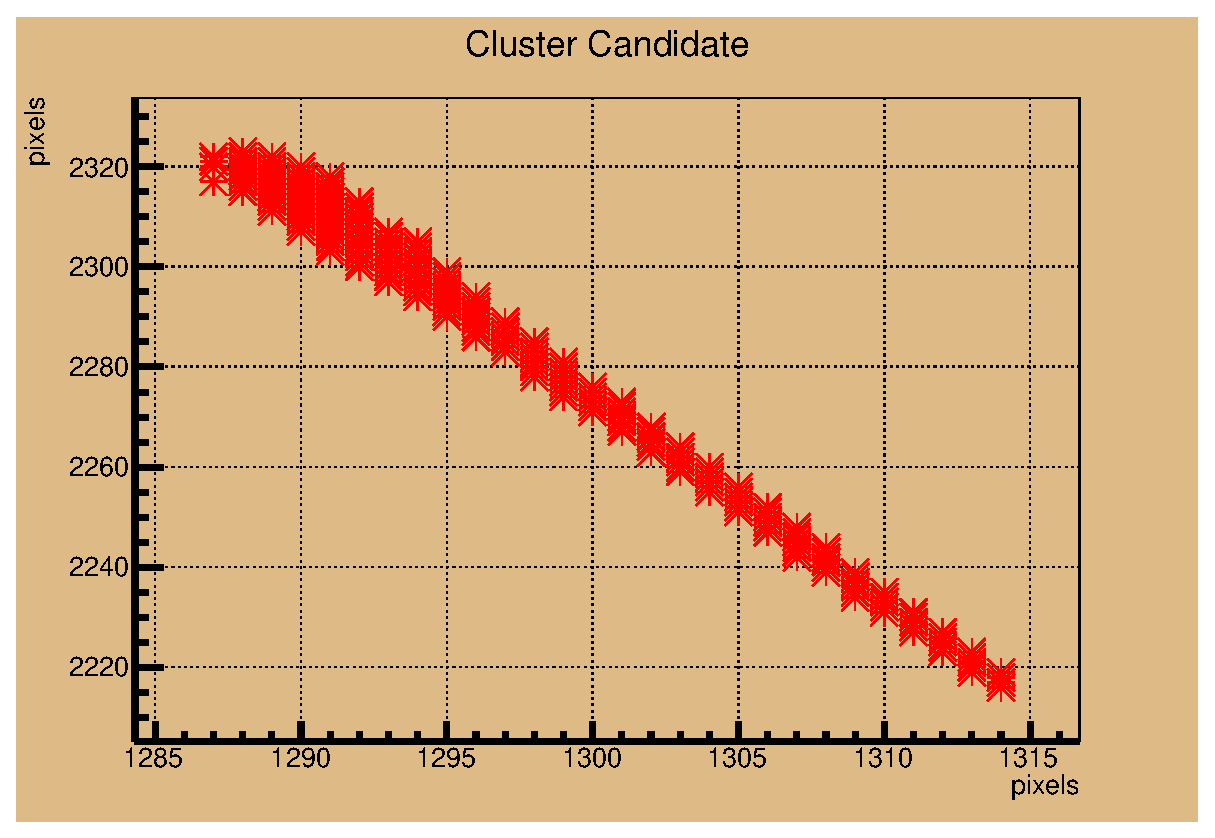
\includegraphics[bb=  100 0 600 350, width=16cm]{/Users/jdeng/baiduCloudDisk/LAMOST/ana/outputs/run1_20171205/20160101/bias/rb-01r-20160101174212-clusterClass.dat_cluster_display_image1_Cluster5_np220_sumpV_131353_graph.eps}
       \caption{A muon candidate found in a raw image of the CCD 01b taken in 20160101.}
       \label{Fig:muon_np220_01b}
   \end{center}    
% ======================================================================
   \end{figure}
% ======================================================================

Fig \ref{Fig:muon_np220_01b} shows a muon candidate event found in the raw image of Fig. \ref{Fig:rawImage_01b}. The muon event has the following attributes: 
%filename =  /Users/jdeng/baiduCloudDisk/LAMOST/ana/outputs/run1_20171205/20160101/bias/rb-01r-20160101174212-clusterClass.dat_cluster_display_image1_Cluster5_np220_sumpV_131353.txt
%data_type =  rb , det =  01r , time_stamp =  20160101174212
%image mean =  0.0 image sstd =  12.2
%image_index =  1
%cluster_index =  5
number of pixels in the cluster =  220 \\
%xmin =  1287
%xmax =  1314
%ymin =  2216
%ymax =  2323
pVmin =  38.6\\
pVmax =  4895.9\\
sumpV =  131354.0\\
avgpV =  597.1\\
correlation coefficient          =  -1.0\\
weighted correlation coefficient =  -1.0\\
eigen values of the covariance matrix=          [  0.55 ,  1014.94 ]\\
weighted eigen values of the covariance matrix= [  0.18 ,  975.01 ]\\


\subsubsection{ROOT Python Package}
To check various distributions, use ROOT Python package for plotting.


% ======================================================================
\subsection{Machine Learning} 
% ======================================================================

% ======================================================================
\subsection{Noise Reduction} 
% ======================================================================

% ======================================================================
\subsection{Energy Calibration} 
% ======================================================================

% ======================================================================
\subsection{MC Simulation and Detection Efficiencies} 
% ======================================================================

% ======================================================================
\section{Preliminary Results} 
% ======================================================================

% ======================================================================
\subsection{Number of Expected Events} 
% ======================================================================

% ======================================================================
\subsection{Statistics and Systematic Uncertainties} 
% ======================================================================

% ======================================================================
\section{Future Prospective: Coming Next...} 
% ======================================================================

% ======================================================================
\subsection{Ultra High Energy Cosmic Rays} 
% ======================================================================

% ======================================================================
\subsection{Ultra High Energy Cosmic Neutrinos} 
% ======================================================================

% ======================================================================
\subsection{Cosmic Neutrinos From the Big Bang} 
% ======================================================================

% ======================================================================
\section{Conclusion} 
% ======================================================================

% ======================================================================
%\section{Reference} 
% ======================================================================

% ======================================================================
   \begin{thebibliography}{99}
% ======================================================================

%    \bibitem{Zgnote} J. Deng et al., \emph{Measurement of $Z\gamma$ Production using 1 $fb^{-1}$ of CDF RUN II Data}, CDF note 8506


% raw data format and astropy module
     \bibitem{astropy} \emph{http://docs.astropy.org/}, Online Astropy Documentation.
     \bibitem{ch-astropy} \emph{http://blog.csdn.net/u013709332/article/details/45768763}, 一个Python用户的天文相关Python资料收集 - 天道酬勤 - 博客频道 - CSDN.NET.

% CCD 
     \bibitem{UCAM-CCD} Lei Jia et al., \emph{The UCAM CCD system of LAMOST}, Proc. SPIE 7733, Ground-based and Airborne Telescopes III, 77335E (7 August 2010); doi: 10.1117/12.856355.


% ======================================================================
   \end{thebibliography}
% ======================================================================


\end{document}
% ======================================================================

